%%%%%%%%%%%%%%%%%%%%%%%%%%%%%%%%%%%%%%%%%%%%%%%%%%%%%%%%%%%%%%%%%%%%%
% University Assignment Title Page 
% LaTeX Template
% Version 1.0 (27/12/12)
%
% This template has been downloaded from:
% http://www.LaTeXTemplates.com
%
% Original author:
% WikiBooks (http://en.wikibooks.org/wiki/LaTeX/Title_Creation)
%
% License:
% CC BY-NC-SA 3.0 (http://creativecommons.org/licenses/by-nc-sa/3.0/)
%%%%%%%%%%%%%%%%%%%%%%%%%%%%%%%%%%%%%%%%%%%%%%%%%%%%%%%%%%%%%%%%%%%%%

\documentclass[11pt,canadien]{article}

\usepackage{babel} % Pour la typo canadienne
\usepackage{graphviz} % Pour inclure des images
\usepackage[utf8]{inputenc} % Pour les accents sur le document
\usepackage{mathptmx} % Pour Times New Roman
\usepackage[top=1in,bottom=1in,left=1in,right=1in]{geometry} % Marges de 1 pouce
\usepackage[toc,page]{appendix} % Pour avoir des annexes et qui figures sur le sommaire
\usepackage{float} % Pour placer précisement les figures (notament la position 'H')
\usepackage{titlesec} % Pour sauter les pages à chaque section

\begin{document}

\newcommand{\sectionbreak}{\clearpage} % Applique le saut de page à chaque section

% Membres du groupe
\newcommand{\antoine}{Antoine \textsc{Moreau}}
\newcommand{\estelle}{Estelle \textsc{Michel}}
\newcommand{\joffrey}{Joffrey \textsc{Germain}}
\newcommand{\julien}{Julien \textsc{Naty-Daufin}}
\newcommand{\karen}{Karen \textsc{Migan}}
\newcommand{\kevin}{Kévin \textsc{Seroux}}
\newcommand{\valentin}{Valentin \textsc{Tertois}}

\begin{titlepage}

\newcommand{\HRule}{\rule{\linewidth}{0.5mm}} % Defines a new command for the horizontal lines, change thickness here

\center % Center everything on the page
 
%-----------------
% HEADING SECTIONS
%-----------------


\includegraphics[width=\textwidth]{images/uqac_logo.jpg} % logo
 
\textsc{\LARGE 8IFG145 - Gestion de projets informatiques}\\[0.5cm]

%--------------
% TITLE SECTION
%--------------

\HRule \\[0.4cm]
{ \huge \bfseries TP1 - Compréhension et exécution de commandes avec GitHub}\\[0.4cm]
\HRule \\[0.5cm]
 
%---------------
% AUTHOR SECTION
%---------------

\begin{minipage}{0.4\textwidth}
\begin{flushleft} \large
\emph{Étudiants :}
\\ \antoine
\\ \estelle
\\ \joffrey
\\ \julien
\\ \karen
\\ \kevin
\\ \valentin
\end{flushleft}
\end{minipage}
~
\begin{minipage}{0.4\textwidth}
\begin{flushright} \large
\emph{Professeur :}\\
Dany \textsc{Fortin-Simard}
\end{flushright}
\end{minipage}\\[2cm]

%-------------
% DATE SECTION
%-------------

{\large \today}\\[2cm]

\vfill % Fill the rest of the page with whitespace

\end{titlepage}

\newpage
\tableofcontents

\section{Introduction au langage Git et à l'outil Github}

\paragraph{} Git est un logiciel créé par Linus Torvalds et dont la première version est sortie le 7 avril 2005. Git a été développé pour linux. C'est un logiciel de gestion de versions gratuit et libre qui permet de gérer des projets de toutes tailles. Plus concrètement, git va permettre de suivre et de gérer l'évolution d'un projet informatique réalisé entre plusieurs personnes de façon simple et efficace. Il va permettre de suivre l'évolution de chaque fichier déposé dans le projet, de garder les anciennes versions de ces fichiers en mémoires, de savoir quel membre du projet a modifié tel ou tel fichier, quand et pourquoi. Git permet également, à deux ou plusieurs personnes, de travailler simultanément sur le même fichier et de fusionner les modifications sans écraser des données. Une des particularités de Git est qu'il repose sur une architecture distribuée. Cela signifie qu'il n'y a pas de serveur central. Chaque personne membre du projet possède l'historique du projet (et donc de chacun des fichiers).

\paragraph{} GitHub est le service d'hébergement web qui utilise le logiciel GitHub. Il est développé par Chris Wanstrath, PJ Hyett et Tom Preston-Werner et a été lancé le 10 avril 2008. De la même façon qu'avec Git, GitHub permet d'héberger et de gérer des projets informatiques. Il permet également une appréhension plus simple du git car il propose une interface graphique pour gérer ces projets au lieu des lignes de commande de Git classique. GitHub permet également une approche plus sociale en intégrant des éléments de communication, de suivi de personne ou de projet.

\section{Apprentissage de Github}
Les commandes \texttt{merge}, \texttt{fetch}, \texttt{pull}, \texttt{push} prennent facultativement en argument le dépôt distant (ex: origin) et la branche distante (ex: master).

\paragraph{git commit}Cette commande est une des commandes principales de l'outil git, elle permet de stocker le contenu de l'index et de "valider" les changements apportés aux fichiers présents dans le dépot. Habituellement, lors de l'exécution de la commande, l'utilisateur utilise l'option \texttt{-m 'Mon texte'} afin de décrire les modifications apportés par cette nouvelle version des fichiers.
\begin{figure}[H]
	\centering
	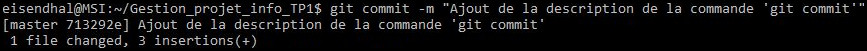
\includegraphics[width=\textwidth]{images/git_commit.jpg}
\end{figure}

\paragraph{git merge}Cette commande permet de fusionner deux branches. Cette commande va fusionner les commits des deux branches depuis leur séparation, le résultat de cette commande est qu'il ne restera plus qu'une branche, intégrant les modifications apportées par les deux branches. L'option \texttt{-m 'Mon texte'} permet de préciser le message du commit qui sera effectué lors de la fusion des deux branches.
\begin{figure}[H]
	\centering
	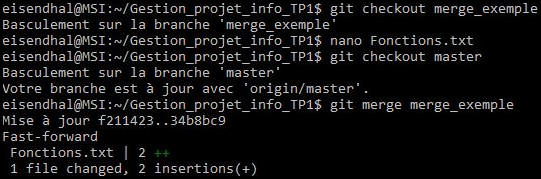
\includegraphics[width=\textwidth]{images/git_merge.jpg}
\end{figure}

\paragraph{git cherry-pick}Cette commande permet d'appliquer les modifications d'un commit particulier d'une autre branche à la branche actuelle. Par exemple, si un correctif a été développé sur une autre branche, et qu'il devient nécessaire de le déployer sur la branche principale, il est possible, grâce à \texttt{cherry-pick}, de ne récupérer que les modifications apportées par le commit qui nous intéresse.
\begin{figure}[H]
	\centering
	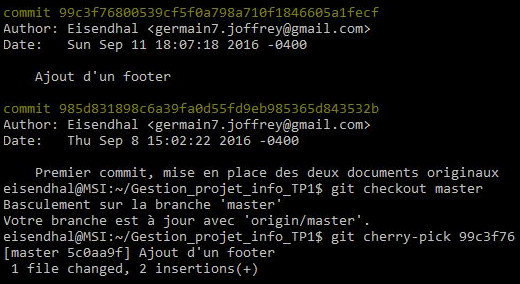
\includegraphics[width=\textwidth]{images/git_cherry-pick.jpg}
\end{figure}

\paragraph{git status}La commande permet d'afficher les chemins qui ont des différences entre le fichier index et le HEAD commit actuel mais aussi les chemins qui ont des différences entre l'arbre actuel et le fichier d'index et enfin les chemins de l'abre actuel qui ne sont pas retenus par GIT. Les premiers chemins correspondent à ce que vous utiliseriez en faisant un \texttt{git commit}, tous les autres correspondent quand à eux à un \texttt{git add} suivi d'un \texttt{git commit}. L'option \texttt{-s} ou \texttt{--short} permet de formater l'affichage de la commande dans le format \texttt{short}.

\paragraph{git log}Permet d'afficher les logs (le journal) des commits. La commande utilise les options applicables à la commande \texttt{git rev-list} afin de contrôler ce qui est affiché et comment, ainsi que les options applicables à la commande \texttt{git diff -*} afin de contrôler l'affichage des changements induits par chaque commit.

\paragraph{git tag}La commande permet de créer, lister, supprimer ou de vérifier un objet "tag" encodé avec la clé GPG. Par exemple si l'on veut supprimer on utilisera  l'option \texttt{-d}, si l'on veut lister on utilisera l'option \texttt{-l} et si l'on veut verifier on utilisera l'option \texttt{-v}.

\paragraph{git branch}La commande permet de gérer tout ce qui a attrait aux branches (ajout, listing, suppression, renommage). On ne peut cependant  pas supprimer une branche qui n'aurait pas été fusionnée avec une autre (on perdrait alors les modifications de la branche). Si on souhaite forcer cette suppression, et perdre tout le travail effectué dessus il faudra utiliser un D majuscule.
\begin{figure}[H]
	\texttt{git branch               \# Permet de lister les branches \\
			git branch <branche>     \# Permet de créer une nouvelle branche <branche> \\
			git branch -m <branche>  \# Renomme la branche courante en <branche> \\
			git branch -d <branche>  \# Permet de supprimer une branche \\
			git branch -D <branche>  \# Supprime la branche même si elle n'a pas été fusionnée
	}
	\begin{figure}[H]
		\centering
		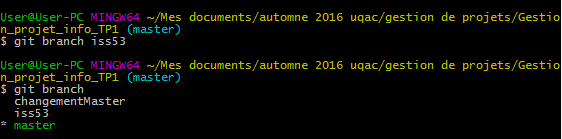
\includegraphics{images/git_branch.png}
	\end{figure}
\end{figure}

\paragraph{git checkout}Une fois les branches créées, il faut être capable d'aller d'une branche à une autre. Pour cela, on peut compter sur la commande \texttt{checkout}. \texttt{git checkout <branche>} permet de se rendre sur une branche existante. En revanche, si vous le souhaitez, vous pouvez demander à git de sauter sur une branche qui n'existe pas en la créant au préalable.
\begin{figure}[H]
	\texttt{git checkout -b <branche> \# est équivalent à : \\
		    git branch <branche> \\
			git checkout <branche>}
	\begin{figure}[H]
		\centering
		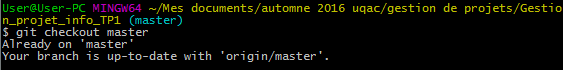
\includegraphics{images/git_checkout.png}
	\end{figure}
\end{figure}

\paragraph{git diff}Comme son nom l’indique, elle permet de voir les changements entre deux versions de fichier (l’ancienne modifiée et l’actuelle) lors de la correction d’un bug ou l’ajout d’une fonctionnalité par exemple. L'option \texttt{--cached} souvent utilisée, permet de comparer après un \texttt{git add} par exemple, les différences avec le dernier commit. Les lignes ajoutées sont donc précédées d’un « + » tandis que les lignes supprimées sont précédées d’un « - ». Normalement les lignes sont colorées et donc faciles à repérer. Par défaut, Git affiche les modifications de tous les fichiers qui ont changé. Vous pouvez demander à Git d’afficher seulement les changements d’un fichier précis, comme ceci : \texttt{git diff chemin/vers/le/fichier.txt}.
\begin{figure}[H]
	\centering
	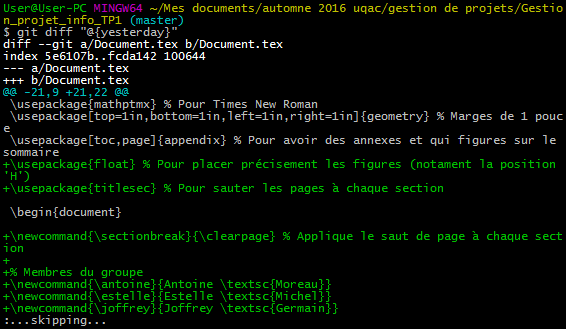
\includegraphics{images/git_diff.png}
\end{figure}

\paragraph{git fetch}Mise à jour des références locales des branches distantes ainsi que des objets git (commit principalement). Dit autrement, elle permet au dépôt local, de prendre simplement conscience des modifications distantes. Elles ne sont pas appliquées aux branches locales. Cette commande est sûre. Par défaut, le dépôt distant \texttt{origin} est fetché mais il est possible d'effectuer cette opération pour tous les dépôts grâce à l'option \texttt{--all}.
\begin{figure}[H]
	\centering
	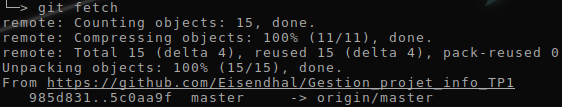
\includegraphics{images/git_fetch.png}
\end{figure}

\paragraph{git pull}Exécution d'un \texttt{git fetch} puis d'un \texttt{git merge}. Bien qu'elle soit pratique, quand la branche locale n'est pas derrière la branche distante, des fusions (avec commits parfois) sont effectués sans pouvoir annuler. Ce qui pose un soucis, pour la lisibilité de l'historique d'un dépôt. Il est d'usage d'utiliser plutôt \texttt{git pull --rebase} afin de remplacer l'opération de merging en une opération de rebasing. Il existe plusieurs façons par \texttt{git config} de spécifier ce comportement par défaut.
\begin{figure}[H]
	\centering
	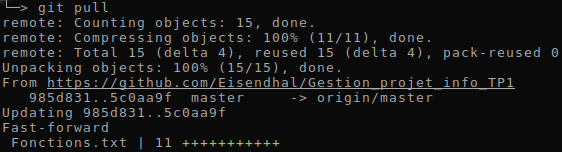
\includegraphics{images/git_pull.png}
\end{figure}

\paragraph{git push}Mise à jour des références du dépôt distant ainsi que des objets git (commit principalement). Dit autrement, elle permet au dépôt distant, d'appliquer les modifications locales. Il pourrait s'agir d'un git pull côté distant, sauf que c'est un autre dépôt qui est à l'initiative. Même si c'est rarement une bonne idée, on peut forcer le push si les branches locales et distantes ne sont pas cohérentes avec l'option \texttt{-f}.
\begin{figure}[H]
	\centering
	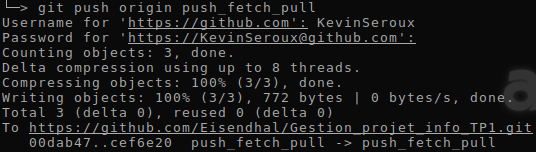
\includegraphics{images/git_push.png}
\end{figure}

\paragraph{git stash}La commande stash permet d'enregistrer l'état actuel du répertoire de travail dans lequel on se trouve (les fichiers modifiés et l'index) dans une pile. Cette commande est particulièrement utile quand on souhaite changer de branche sur un projet alors que les modifications que l'on a apportées aux fichiers sont en conflit avec le répertoire source. Dans ce cas, la commande \texttt{git pull} ne va pas autoriser la réécriture. Pour résoudre ce problème, on peut effectuer un \texttt{git stash} pour stocker les changements en cours et partir travailler dans une autre branche. Il suffit ensuite de faire \texttt{git stash --list} pour afficher la liste de toutes les stashs enregistrées. Pour recharger la dernière stash effectuée il faut entrer la commande \texttt{git stash apply}. Si l'on veut charger une stash antérieur, il faut préciser lequel en utilisant la commande \texttt{git stash apply stash@{X}} (X étant le numéro de la stash que l'on veut sélectionner).
\begin{figure}[H]
	\centering
	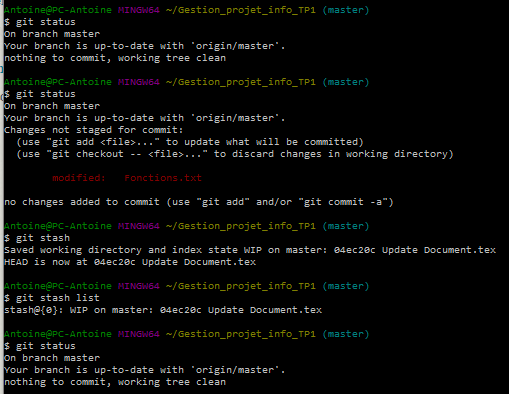
\includegraphics{images/git_stash.png}
\end{figure}

\paragraph{git reset}La commande reset permet de corriger des erreurs dans l'arbre de travail dans lequel on se situe. Pour ce faire reset va réinitialiser l'arbre de travail dans l'état auquel il était au dernier commit. Il faut noté que la commande reset va corriger uniquement des erreurs qui n'ont pas été commit. En utilisant la commande \texttt{git reset --hard HEAD} à la fois toutes les modifications faites sur l'arbre ainsi que les modifications de l'index git seront supprimées.
\begin{figure}[H]
	\centering
	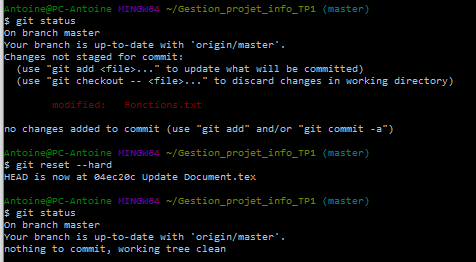
\includegraphics{images/git_reset.png}
\end{figure}

\paragraph{git init}Cette commande permet de créer un répertoire git vide contenant les sous répertoires refs/heads et refs/tags. Cette fonction ne peut pas être lancée dans un répertoire existant. On peut notamment l’utiliser de la façon suivante : \texttt{git init –q}, où \texttt{–q} permet de supprimer l’affichage de tous les messages concernant la réalisation de la commande, à l’exception des messages d’erreur.

\paragraph{git clone}Cette commande permet créer un nouveau répertoire identique à celui placé en argument. On peut utiliser cette commande avec l’option \texttt{-l} : on obtient \texttt{git clone -l "le nom du répertoire"}, où \texttt{-l} permet de de créer ce clone directement dans la mémoire interne de la machine.

\paragraph{git rebase}Cette commande permet d'ajouter toutes les modifications faites sur une branche, à une autre branche. On peut utiliser cette commande avec l'option \texttt{–onto} : on obtient \texttt{git rebase –onto "nom du fichier"}, où \texttt{–onto} permet de choisir à partir de quel fichier d'une branche les modification d'une autre branche sont ajoutées.

\paragraph{git add} ajoute les modifications d’un fichier de la branche active dans le dépôt de git. Elle est utilisée avant le commit. \texttt{–p} : on obtient \texttt{git add –p "nom du fichier"}, où \texttt{–p} (patch mode) Elle est utilisée pour les fichiers modifiés. Cette option permet d’indexer les modifications que l’on souhaite retenir ou les indexer séparément. Il y a plusieurs modes : indexer, ne pas indexer, indexer le reste des modifications, etc.

\paragraph{git rm} rm filesource  newfile : permet d’effacer un fichier de la branche courante et de l’ index. \texttt{–-cached} : on obtient \texttt{git rm --cached "nom du fichier"}, où \texttt{–-cached} supprime le fichier du dépôt git mais pas du répertoire personnel.

\paragraph{git mv} renomme un fichier et/ou le change de répertoire. \texttt{–f} : on obtient \texttt{git rm -f "nom du fichier"}, où \texttt{–f} force le renommage du fichier ou son déplacement. Il peut être dangereux car les fichiers du même nom sont effacés. 

\section{Utilisation de Github}
Blablabla

\newpage
\begin{appendices} % Les annexes commencent

\section{Répartition des différentes tâches}
\begin{tabular}{l l l l}
	\textbf{Tâche} & \textbf{Temps} & \textbf{Date d'échéance} & \textbf{Responsable}
	\\ \hline
	   Partie 2 - Présentation de Git       & 3h    & 2016-09-22 & \antoine
	\\ Mise en forme du document final      & 3h    & 2016-10-04 & \kevin
	\\ Mise en place du dépôt Git et droits & 45min & 2016-09-08 & \joffrey
	\\ Description \texttt{git add}         & 30min & 2016-09-15 & \estelle
	\\ Description \texttt{git mv}          & 30min & 2016-09-15 & \estelle
	\\ Description \texttt{git rm}          & 30min & 2016-09-15 & \estelle
	\\ Description \texttt{git init}        & 30min & 2016-09-15 & \julien
	\\ Description \texttt{git clone}       & 30min & 2016-09-15 & \julien
	\\ Description \texttt{git rebase}      & 30min & 2016-09-15 & \julien
	\\ Description \texttt{git status}      & 30min & 2016-09-15 & \valentin
	\\ Description \texttt{git log}         & 30min & 2016-09-15 & \valentin
	\\ Description \texttt{git tag}         & 30min & 2016-09-15 & \valentin
	\\ Description \texttt{git commit}      & 30min & 2016-09-15 & \joffrey
	\\ Description \texttt{git merge}       & 30min & 2016-09-15 & \joffrey
	\\ Description \texttt{git cherry-pick} & 30min & 2016-09-15 & \joffrey
	\\ Description \texttt{git diff}        & 30min & 2016-09-15 & \karen
	\\ Description \texttt{git branch}      & 30min & 2016-09-15 & \karen
	\\ Description \texttt{git checkout}    & 30min & 2016-09-15 & \karen
	\\ Description \texttt{git push}        & 30min & 2016-09-15 & \kevin
	\\ Description \texttt{git fetch}       & 30min & 2016-09-15 & \kevin
	\\ Description \texttt{git pull}        & 30min & 2016-09-15 & \kevin
	\\ Description \texttt{git stash}       & 30min & 2016-09-15 & \antoine
	\\ Description \texttt{git reset}       & 30min & 2016-09-15 & \antoine
	\\ \ldots
	\\ Correction orthographique du rapport & 1h    & 2016-10-04 & Grammar Nazi (Joffrey)
	\\ Évaluation du groupe                 & 45min & \ldots     & Tous
	\\ Présentation orale                   & 5min  & 2016-10-04 & Estelle, Julien, Valentin
\end{tabular}

\section{Évaluation des membres}
Blablabla

\end{appendices}

\end{document}
